Quantum information with a twist at quantum money.
\begin{parts}
	\part Description of quantum states after measurement:
	\begin{subparts}
		\subpart After measurement, Alice will get one of the 2 basis states, thus $\rho_\textnormal{A}$ is either $\ket{0}\bra{0}$ or $\ket{1}\bra{1}$.
		\subpart However Bob has no information on the measurement result, therefore the best he can do is to encode the decoherence with $\rho_\textnormal{B} = |\alpha|^2 \ket{0}\bra{0} + |\beta|^2 \ket{1}\bra{1}$.
	\end{subparts}
	
	The difference is that while Alice has the deterministic result of her measurement, Bob can only observe the decoherence and thus has the results probabilistically mixed in $\rho_\textnormal{B}$ -- similar to what one does to account for unintentional measurement in a quantum system.
	
	\part
	\begin{subparts}
		\subpart We know that Hadamard gate transforms between $\ket{0} \leftrightarrow \ket{+}$ and $\ket{1} \leftrightarrow \ket{-}$, thus we have the following network for X basis measurement:
		\begin{figure}[H]
			\centering
			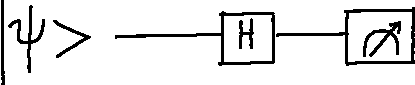
\includegraphics[width=.35\linewidth, trim=0 3em 0 2em]{q4-x-measure}
		\end{figure}
		
		\begin{align*}
			\ket{\psi} &= \alpha \ket{0} + \beta \ket{1} \\
			&= \alpha \rbracket{\frac{\ket{+} + \ket{-}}{\sqrt{2}}} + \beta \rbracket{\frac{\ket{+} - \ket{-}}{\sqrt{2}}} \\
			&= \frac{\alpha + \beta}{\sqrt{2}}\ket{+} \;+\; \frac{\alpha - \beta}{\sqrt{2}}\ket{-} \\[1em]
			\Rightarrow P(+) &= \abs{\frac{\alpha + \beta}{\sqrt{2}}}^2 = \frac{1}{2} \abs{\alpha + \beta}^2 \\
			P(-) &= \frac{1}{2} \abs{\alpha - \beta}^2
		\end{align*}
		
		\subpart Realise that after measurement, Alice would have a pure state of $\ket{+}$ or $\ket{-}$, either containing $(\ket{0}\pm\ket{1}) / \sqrt{2} \Rightarrow P(0)=P(1)=\diagfrac{1}{2}$ after X measurement.
		
		From Bob's perspective, we then have the tree diagram:
		\begin{figure}[H]
			\centering
			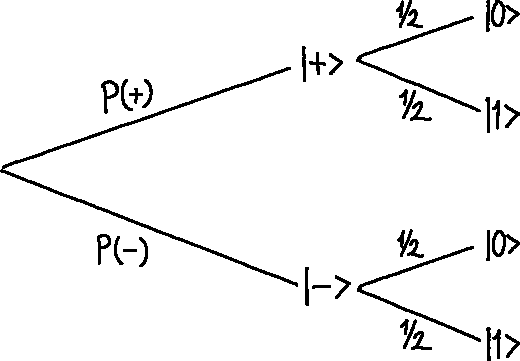
\includegraphics[width=.45\linewidth]{q4-bob-tree}
		\end{figure}
		
		Thus $\rho_\textnormal{B}$ is now:
		\begin{align*}
			&\frac{P(+)+P(-)}{2} \ket{0}\bra{0} + \frac{P(+)+P(-)}{2} \ket{1}\bra{1} \\
			&\qquad = \frac{1}{4} \Bigl[|\alpha|^2 + |\beta|^2 + \alpha^* \beta + \beta^* \alpha + |\alpha|^2 + |\beta|^2 - \alpha^* \beta - \beta^* \alpha\Bigr] \bigl[\ket{0}\bra{0} + \ket{1}\bra{1}\bigr] \\
			&\qquad = \frac{1}{2} \bigl[\ket{0}\bra{0} + \ket{1}\bra{1}\bigr]
		\end{align*}
	\end{subparts}
	
	\part
	\begin{subparts}
		\subpart As Calvin has no information on $\ket{\psi}$, he can only construct $\rho_\textnormal{C} = \textnormal{diag}(|\alpha|^2,\,|\beta|^2)$ in Z basis. Hence fidelity:
		\begin{align*}
			\mathcal{F} &= \bra{\psi}\rho_\textnormal{C}\ket{\psi} \\
			&= |\alpha|^4 + |\beta|^4 \\
			&= 2|\alpha|^4 - 2|\alpha|^2 + 1
		\end{align*}
		
		\subpart Note if $\ket{\psi}$ is either $\ket{0}$ or $\ket{1}$, we have $\mathcal{F}=1 \Leftarrow$ maximum fidelity states.
		
		\subpart But if $|\alpha|=|\beta|=\diagfrac{1}{\sqrt{2}}$, i.e. $\ket{\psi}$ lies on the equator of the Bloch sphere, we have $|\alpha|^2 = \diagfrac{1}{2} \Rightarrow \mathcal{F}=\diagfrac{1}{2}$.
		
		\subpart Thus average fidelity is $\langle \mathcal{F} \rangle = \diagfrac{1}{3}\mathcal{F}_z + \diagfrac{1}{3}\mathcal{F}_x + \diagfrac{1}{3}\mathcal{F}_y = \diagfrac{1}{3}\times 1 + \diagfrac{2}{3}\times\frac{1}{2} = \diagfrac{2}{3}$.
	\end{subparts}
	
	\part For each qubit, $P(\textnormal{Alice having Z})=\diagfrac{1}{2}$ and note that even for the wrong basis, we have a probability of $\diagfrac{1}{2}$ of getting the right value.
	\begin{subparts}
		\subpart Thus we have:
		\begin{equation*}
			P(\textnormal{correct value}|\textnormal{measure Z constantly}) = \underbracket{\frac{1}{2}}_{\substack{\textnormal{right}\\\textnormal{basis}}} + \underbracket{\frac{1}{2}}_{\substack{\textnormal{wrong}\\\textnormal{basis}}}\times\underbracket{\frac{1}{2}}_{\substack{\textnormal{but still get}\\\textnormal{the correct value}}} = \frac{3}{4}
		\end{equation*}
		
		\subpart With reference to the tree diagram below, we have:
		\begin{figure}[H]
			\centering
			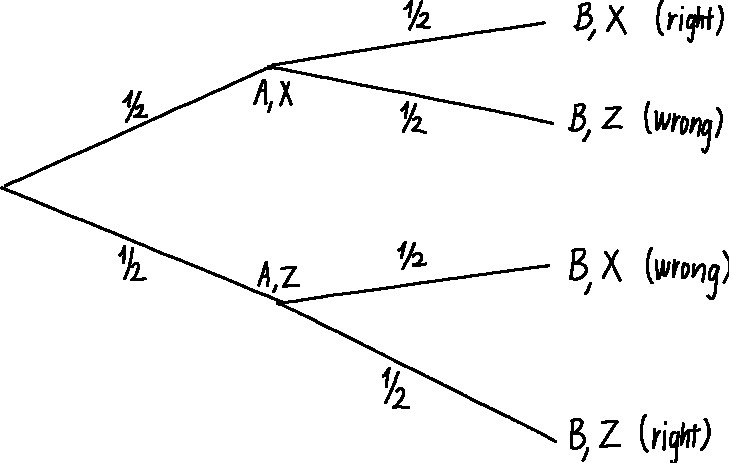
\includegraphics[width=.5\linewidth]{q4-money-tree}
		\end{figure}
		\begin{gather*}
			P(\textnormal{correct value}|\textnormal{X, Z at random}) = 2\underbracket{(\frac{1}{2}\times\frac{1}{2})}_{\textnormal{right basis}} + 2\underbracket{(\frac{1}{2}\times\frac{1}{2}\times\frac{1}{2})}_{\substack{\textnormal{wrong basis}\\\textnormal{but right value}}} \\
			= \frac{1}{2} + \frac{1}{4} = \frac{3}{4}
		\end{gather*}
	\end{subparts}
	
	\part
	\begin{subparts}
		\subpart For Alice to detect the forgery, she needs to obtain the wrong value so we have for every bit:
		\begin{equation*}
			P(\textnormal{wrong value}\cap\textnormal{wrong basis}) = \frac{1}{2}\times\frac{1}{2} = \frac{1}{4}
		\end{equation*}
		
		For $n=24$ we have:
		\begin{align*}
			P(\textnormal{detection}) &= 1-P(\textnormal{no wrong value}) \\
			&= 1 - \rbracket{\frac{3}{4}}^n \\
			&= 0.999
		\end{align*}
		
		\subpart If Daisy has access to the original banknote, the best she could do is to gain knowledge of some of her basis being incorrect as per the $\diagfrac{1}{4}$ probability above.
		
		By no-cloning theorem, she is unable to copy the note either -- measurement would also collapse the state into her measurement basis and render the note useless for further probing.
	\end{subparts}
\end{parts}